%\documentclass[portrait,final,a0paper]{baposter}
\documentclass[paperwidth=48in,paperheight=48in,portrait,final]{baposter}
% Usa a4shrink for an a4 sized paper.

\tracingstats=2

\usepackage{calc}
\usepackage{graphicx}
\usepackage{amsmath}
\usepackage{amssymb}
\usepackage{latexsym}
\usepackage{relsize}
\usepackage{multirow}
\usepackage{bm}

\usepackage{graphicx}
\usepackage{multicol}


\usepackage{pgfbaselayers}
\pgfdeclarelayer{background}
\pgfdeclarelayer{foreground}
\pgfsetlayers{background,main,foreground}

\usepackage{times}
%\usepackage{helvet}
%\usepackage{bookman}
\usepackage{palatino}

\newcommand{\captionfont}{\footnotesize}

\selectcolormodel{cmyk}

\graphicspath{{images/}}

%%%%%%%%%%%%%%%%%%%%%%%%%%%%%%%%%%%%%%%%%%%%%%%%%%%%%%%%%%%%%%%%%%%%%%%%%%%%%%%%
%%%% Some math symbols used in the text
%%%%%%%%%%%%%%%%%%%%%%%%%%%%%%%%%%%%%%%%%%%%%%%%%%%%%%%%%%%%%%%%%%%%%%%%%%%%%%%%
% Format 
\newcommand{\Matrix}[1]{\begin{bmatrix} #1 \end{bmatrix}}
\newcommand{\Vector}[1]{\Matrix{#1}}
\newcommand*{\SET}[1]  {\ensuremath{\mathcal{#1}}}
\newcommand*{\MAT}[1]  {\ensuremath{\mathbf{#1}}}
\newcommand*{\VEC}[1]  {\ensuremath{\bm{#1}}}
\newcommand*{\CONST}[1]{\ensuremath{\mathit{#1}}}
\newcommand*{\norm}[1]{\mathopen\| #1 \mathclose\|}% use instead of $\|x\|$
\newcommand*{\abs}[1]{\mathopen| #1 \mathclose|}% use instead of $\|x\|$
\newcommand*{\absLR}[1]{\left| #1 \right|}% use instead of $\|x\|$

\def\norm#1{\mathopen\| #1 \mathclose\|}% use instead of $\|x\|$
\newcommand{\normLR}[1]{\left\| #1 \right\|}% use instead of $\|x\|$

%%%%%%%%%%%%%%%%%%%%%%%%%%%%%%%%%%%%%%%%%%%%%%%%%%%%%%%%%%%%%%%%%%%%%%%%%%%%%%%%
% Multicol Settings
%%%%%%%%%%%%%%%%%%%%%%%%%%%%%%%%%%%%%%%%%%%%%%%%%%%%%%%%%%%%%%%%%%%%%%%%%%%%%%%%
\setlength{\columnsep}{0.7em}
\setlength{\columnseprule}{0mm}


%%%%%%%%%%%%%%%%%%%%%%%%%%%%%%%%%%%%%%%%%%%%%%%%%%%%%%%%%%%%%%%%%%%%%%%%%%%%%%%%
% Save space in lists. Use this after the opening of the list
%%%%%%%%%%%%%%%%%%%%%%%%%%%%%%%%%%%%%%%%%%%%%%%%%%%%%%%%%%%%%%%%%%%%%%%%%%%%%%%%
\newcommand{\compresslist}{%
\setlength{\itemsep}{1pt}%
\setlength{\parskip}{0pt}%
\setlength{\parsep}{0pt}%
}


%%%%%%%%%%%%%%%%%%%%%%%%%%%%%%%%%%%%%%%%%%%%%%%%%%%%%%%%%%%%%%%%%%%%%%%%%%%%%%
%%% Begin of Document
%%%%%%%%%%%%%%%%%%%%%%%%%%%%%%%%%%%%%%%%%%%%%%%%%%%%%%%%%%%%%%%%%%%%%%%%%%%%%%

\begin{document}

%%%%%%%%%%%%%%%%%%%%%%%%%%%%%%%%%%%%%%%%%%%%%%%%%%%%%%%%%%%%%%%%%%%%%%%%%%%%%%
%%% Here starts the poster
%%%---------------------------------------------------------------------------
%%% Format it to your taste with the options
%%%%%%%%%%%%%%%%%%%%%%%%%%%%%%%%%%%%%%%%%%%%%%%%%%%%%%%%%%%%%%%%%%%%%%%%%%%%%%
% Define some colors
\definecolor{silver}{cmyk}{0,0,0,0.3}
\definecolor{yellow}{cmyk}{0,0,0.9,0.0}
\definecolor{reddishyellow}{cmyk}{0,0.22,1.0,0.0}
\definecolor{black}{cmyk}{0,0,0.0,1.0}
\definecolor{darkYellow}{cmyk}{0,0,1.0,0.5}
\definecolor{darkSilver}{cmyk}{0,0,0,0.1}

\definecolor{lightyellow}{cmyk}{0,0,0.3,0.0}
\definecolor{lighteryellow}{cmyk}{0,0,0.1,0.0}
\definecolor{lightestyellow}{cmyk}{0,0,0.05,0.0}

% http://www.creativecolorschemes.com/resources/free-color-schemes/blue-tone-color-scheme.shtml

\definecolor{colorA}{cmyk}{1,0.25,0.1,0.5}
\definecolor{colorB}{cmyk}{1,0.3,0.05,0.2}
\definecolor{colorC}{cmyk}{0.6,0,0.05,0}
\definecolor{colorD}{cmyk}{0.95,0.6,0.05,0.15}
\definecolor{colorE}{cmyk}{0.6,0.3,0.05,0.05}
\definecolor{colorF}{cmyk}{0.4,0.15,0,0}
\definecolor{colorf}{cmyk}{0.1,0.0375,0,0}
\definecolor{colorG}{cmyk}{0.75,0.3,0.05,0.1}
\definecolor{colorH}{cmyk}{0.65,0.15,0,0.05}
\definecolor{colorI}{cmyk}{0.3,0.05,0,0}
\definecolor{colorJ}{cmyk}{0.65,0,1,0}
\definecolor{colorK}{cmyk}{0,0.5,1,0}
\definecolor{colork}{cmyk}{0,0.125,0.25,0}
\definecolor{colorL}{cmyk}{0.65,0.8,0,0}
\definecolor{colorM}{cmyk}{0.7,0.4,0.2,0.6}
\definecolor{colorN}{cmyk}{0.3,0.15,0.1,0.3}
\definecolor{colorn}{cmyk}{0.075,0.0375,0.025,0.075}
\definecolor{colorO}{cmyk}{0.25,0.05,0.1,0.15}

%%
\typeout{Poster Starts}
\background{
  \begin{tikzpicture}[remember picture,overlay]%
    \draw (current page.north west)+(-2em,2em) node[anchor=north west] {\includegraphics[height=1.1\textheight]{silhouettes_background}};
  \end{tikzpicture}%
}

\newlength{\leftimgwidth}
\begin{poster}%
  % Poster Options
  {
  % Show grid to help with alignment
  grid=no,
  % Column spacing
  colspacing=1em,
  % Color style
  bgColorOne=colorf,
  bgColorTwo=white,
  borderColor=colorK,
  headerColorOne=colork,
  headerColorTwo=white,
  headerFontColor=colorM,
  boxColorOne=white,
  boxColorTwo=colorC,
  % Format of textbox
  textborder=roundedleft,
%  textborder=rectangle,
  % Format of text header
  eyecatcher=no,
  headerborder=closed,
  headerheight=0.11\textheight,
  headershape=roundedright,
  headershade=shade-lr,
  headerfont=\Large, %Sans Serif
  boxshade=plain,
%  background=shade-tb,
  background=plain,
  linewidth=2pt
  }
  % Eye Catcher
  {\includegraphics[width=10em]{D1077}} % No eye catcher for this poster. (eyecatcher=no above). If an eye catcher is present, the title is centered between eye-catcher and logo.
  % Title
  { %Sans Serif
  %\bf% Serif
  Multivariate analysis of diffusion tensor imaging and cortical thickness maps in a traumatic brain injury (TBI) cohort using Advanced Normalization Tools (ANTs)
  \vspace{0.1em}}
  % Authors
  { %Sans Serif
  % Serif
  Nicholas J. Tustison$^1$, Brian B. Avants$^2$, Philip A. Cook$^2$, Junghoon Kim$^3$, John Whyte$^3$, James C. Gee$^2$, Stephen  Ahlers$^4$, James R. Stone$^1$ \newline
  % Affiliations
  {\normalsize $^1$University of Virginia, $^2$University of Pennsylvania, $^3$Moss Rehabilitation Research Institute, $^4$Naval Medical Research Center \\
  P309
  }
  
  }
  % University logo
  {% The makebox allows the title to flow into the logo, this is a hack because of the L shaped logo.
%    \makebox[8em][r]{%
%      \begin{minipage}{16em}
%        \hfill
%%        \includegraphics[height=2em]{msrlogo}
%        \includegraphics[height=7.0em]{logo}
%      \end{minipage}
%    }
  }

  \tikzstyle{light shaded}=[top color=baposterBGtwo!30!white,bottom color=baposterBGone!30!white,shading=axis,shading angle=30]

  % Width of left inset image
     \setlength{\leftimgwidth}{0.78em+8.0em}

%%%%%%%%%%%%%%%%%%%%%%%%%%%%%%%%%%%%%%%%%%%%%%%%%%%%%%%%%%%%%%%%%%%%%%%%%%%%%%
%%% Now define the boxes that make up the poster
%%%---------------------------------------------------------------------------
%%% Each box has a name and can be placed absolutely or relatively.
%%% The only inconvenience is that you can only specify a relative position 
%%% towards an already declared box. So if you have a box attached to the 
%%% bottom, one to the top and a third one which should be in between, you 
%%% have to specify the top and bottom boxes before you specify the middle 
%%% box.
%%%%%%%%%%%%%%%%%%%%%%%%%%%%%%%%%%%%%%%%%%%%%%%%%%%%%%%%%%%%%%%%%%%%%%%%%%%%%%
    %
    % A coloured circle useful as a bullet with an adjustably strong filling
    \newcommand{\colouredcircle}[1]{%
      \tikz{\useasboundingbox (-0.2em,-0.32em) rectangle(0.2em,0.32em); \draw[draw=black,fill=baposterBGone!80!black!#1!white,line width=0.03em] (0,0) circle(0.18em);}}

%%%%%%%%%%%%%%%%%%%%%%%%%%%%%%%%%%%%%%%%%%%%%%%%%%%%%%%%%%%%%%%%%%%%%%%%%%%%%%
  \headerbox{Introduction}{name=introduction,column=0,row=0}{
%%%%%%%%%%%%%%%%%%%%%%%%%%%%%%%%%%%%%%%%%%%%%%%%%%%%%%%%%%%%%%%%%%%%%%%%%%%%%%

TBI is a complex disease process involving mechanical disruption
of neurological tissues and activation of secondary injury cascades, 
culminating in loss of function.  Multiple neuroimaging approaches 
have recently been developed to detect white matter (WM) and gray 
matter injury following TBI. 
%Diffusion tensor imaging (DTI) affords 
%quantification of microstructural white matter injury. High-resolution 
%T1-weighted sequences allow for computation of cortical thickness maps. 
It is hypothesized that a multivariate analysis of these two imaging 
modalities may provide insight into the alteration of cortical and WM 
circuits following TBI.  To address this hypothesis, we employ a novel 
multivariate technique, sparse canonical correlation analysis (SCCA), 
to quantify traumatically induced disruption of WM and cortical networks.

  \vspace{0.3em}
 }

%%%%%%%%%%%%%%%%%%%%%%%%%%%%%%%%%%%%%%%%%%%%%%%%%%%%%%%%%%%%%%%%%%%%%%%%%%%%%%
  \headerbox{Diffuse traumatic brain injury data}{name=data,column=0,below=introduction}{
%%%%%%%%%%%%%%%%%%%%%%%%%%%%%%%%%%%%%%%%%%%%%%%%%%%%%%%%%%%%%%%%%%%%%%%%%%%%%%
The TBI data used in this study is part of a larger effort investigating 
the relationship between various neuroimaging indices and cognitive and 
functional abilities in long-term survivors of TBI (principal 
investigator: John Whyte).   
\paragraph{Description of cohort: }
17 controls and 16 patients with TBI were used.  
Each patient had a history of non-penetrating traumatic brain injury 
of at least moderate severity defined by significant and well-documented
loss or alteration of consciousness following injury in addition to meeting
several other exclusionary criteria.  The healthy volunteers were matched in terms of age, gender, ethnicity, handedness, and years of education.
\paragraph{Image acquisition:} 
High resolution T1-weighted anatomic images were obtained using a 3D MP-RAGE 
imaging sequence with the following acquisition parameters: TR = 1620 ms, 
TI = 950 ms, TE = 3 ms, flip angle = 15$^\circ$, 160 contiguous slices of 
1.0 mm thickness, FOV = 192 $\times$ 256 mm$^2$, matrix = 192 $\times$ 256, 
1NEX with a scan time of 6 minutes, and voxel size = 1 mm$^3$.  30-directional
DTI images were also obtained. 
    
      \vspace{0.3em}
  }

%%%%%%%%%%%%%%%%%%%%%%%%%%%%%%%%%%%%%%%%%%%%%%%%%%%%%%%%%%%%%%%%%%%%%%%%%%%%%%
  \headerbox{Advanced Normalization Tools}{name=ants,column=0,span=1,below=data,above=bottom}{
%%%%%%%%%%%%%%%%%%%%%%%%%%%%%%%%%%%%%%%%%%%%%%%%%%%%%%%%%%%%%%%%%%%%%%%%%%%%%%
%\begin{itemize}
%\item{\bf Processing}
%\vspace{-10mm}\\
\begin{center}
{\bf Processing} \\
\vspace{2mm}
\begin{tabular}{cc}
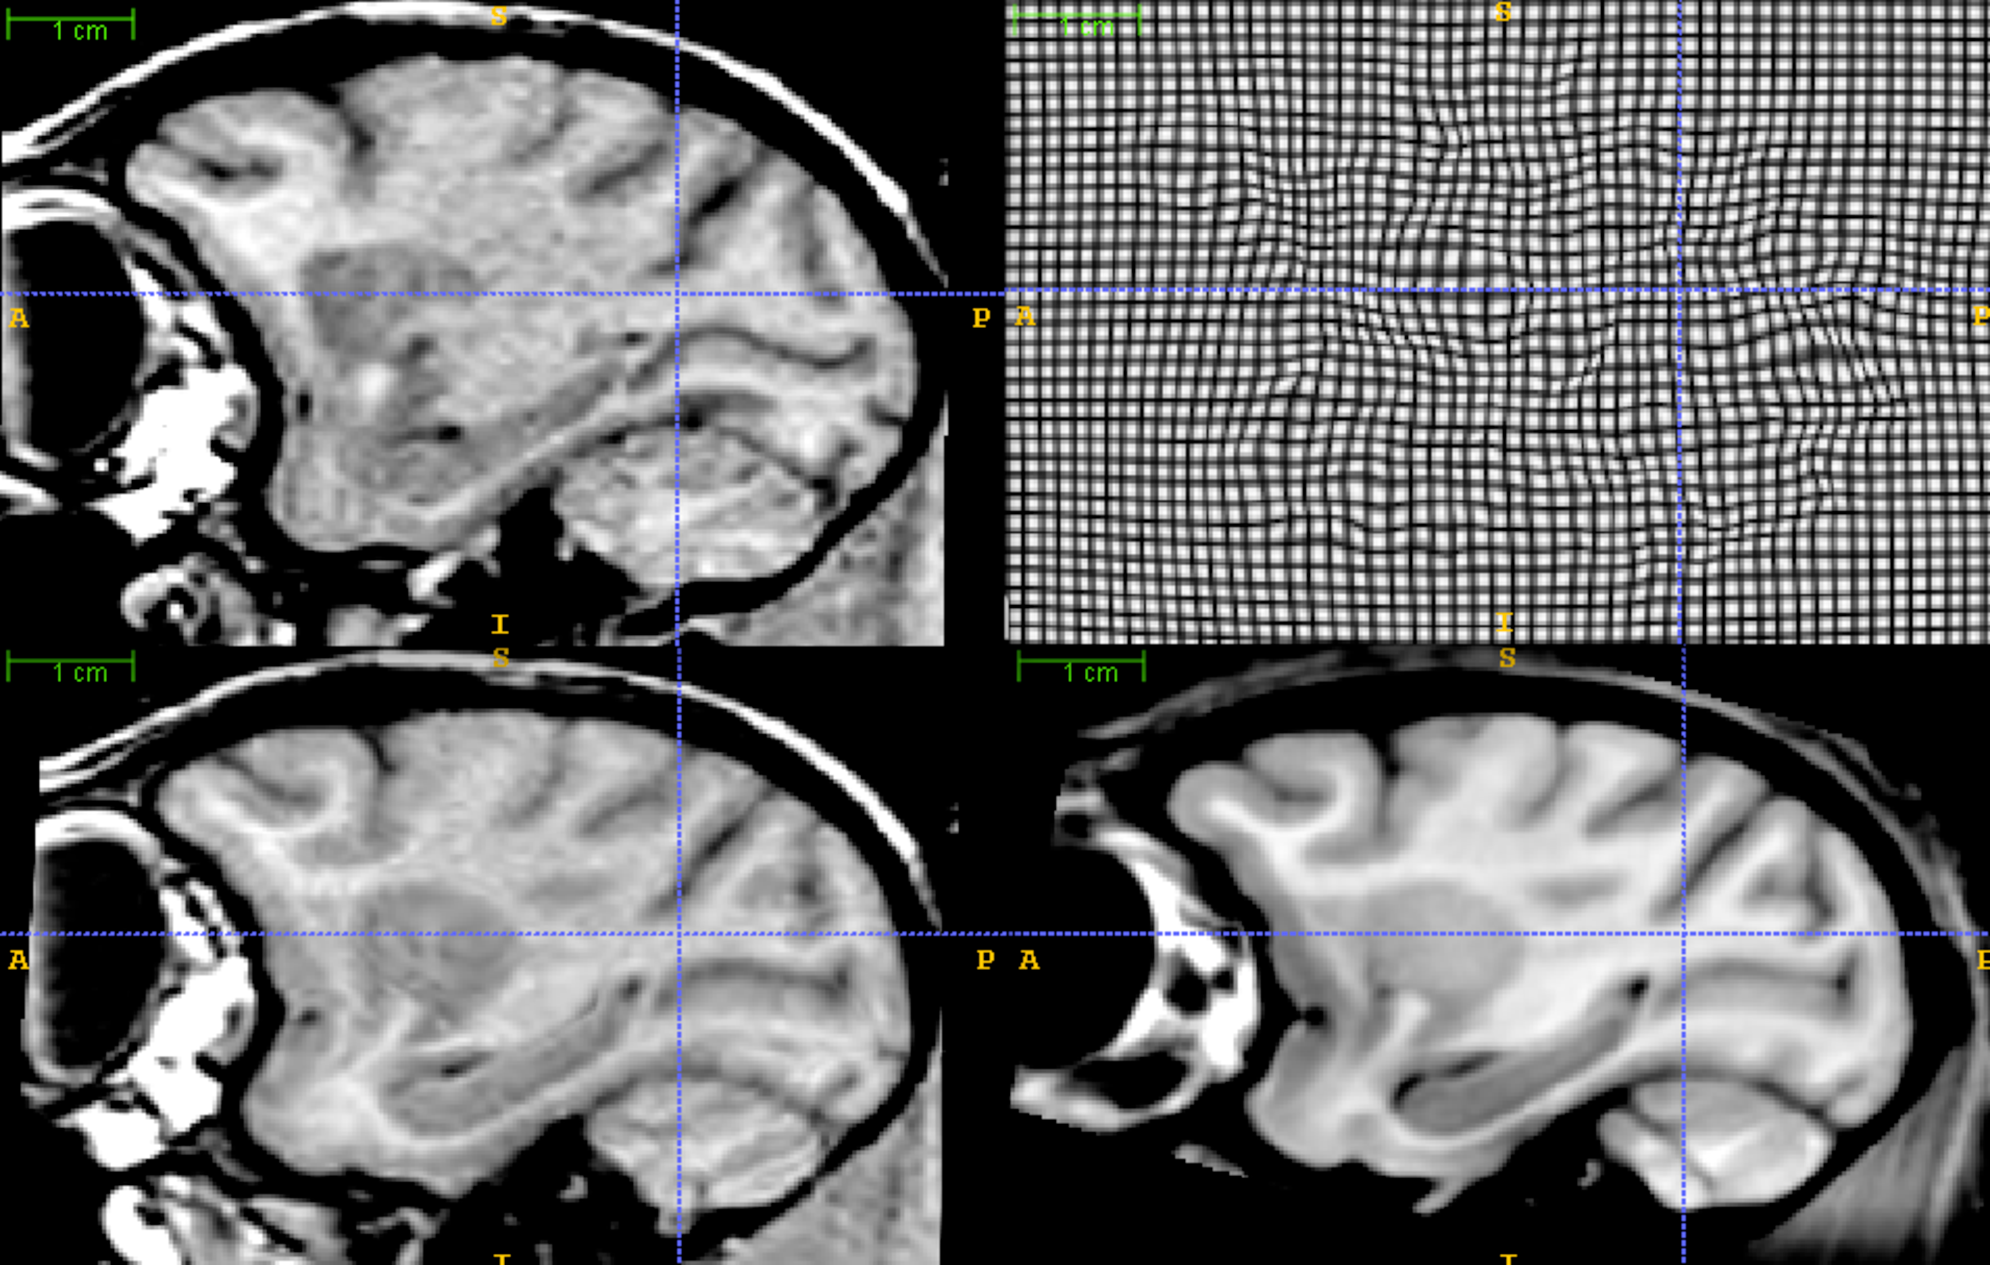
\includegraphics[height=20mm]{normalization.pdf} & 
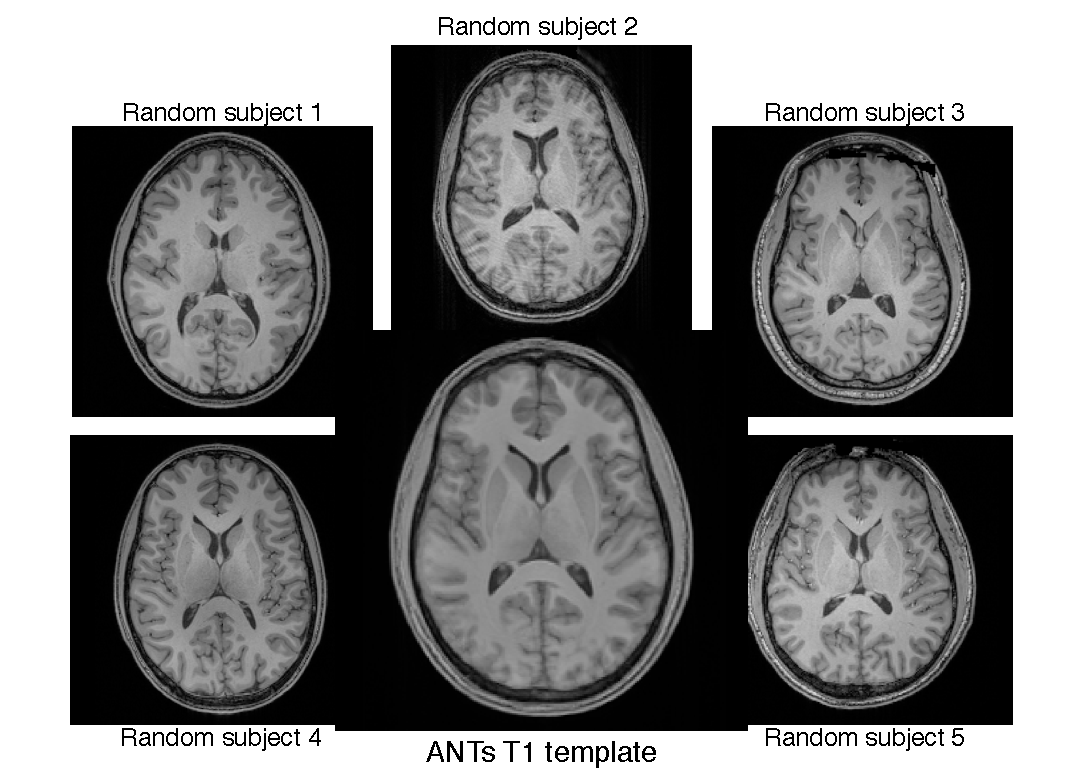
\includegraphics[height=25mm]{template.pdf} \\
SyN normalization \cite{Avants2011} & SyGN template building \cite{Avants2010}\\
\vspace{-1mm}\\
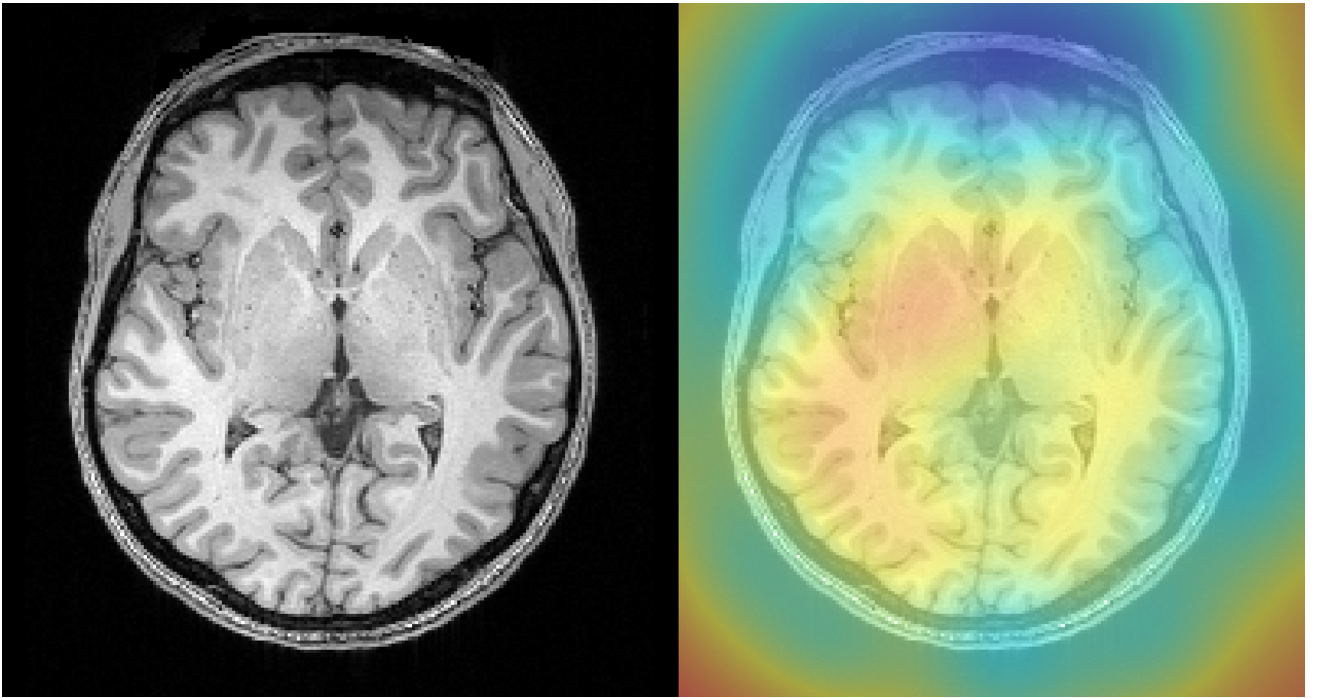
\includegraphics[height=20mm]{n4.pdf} & 
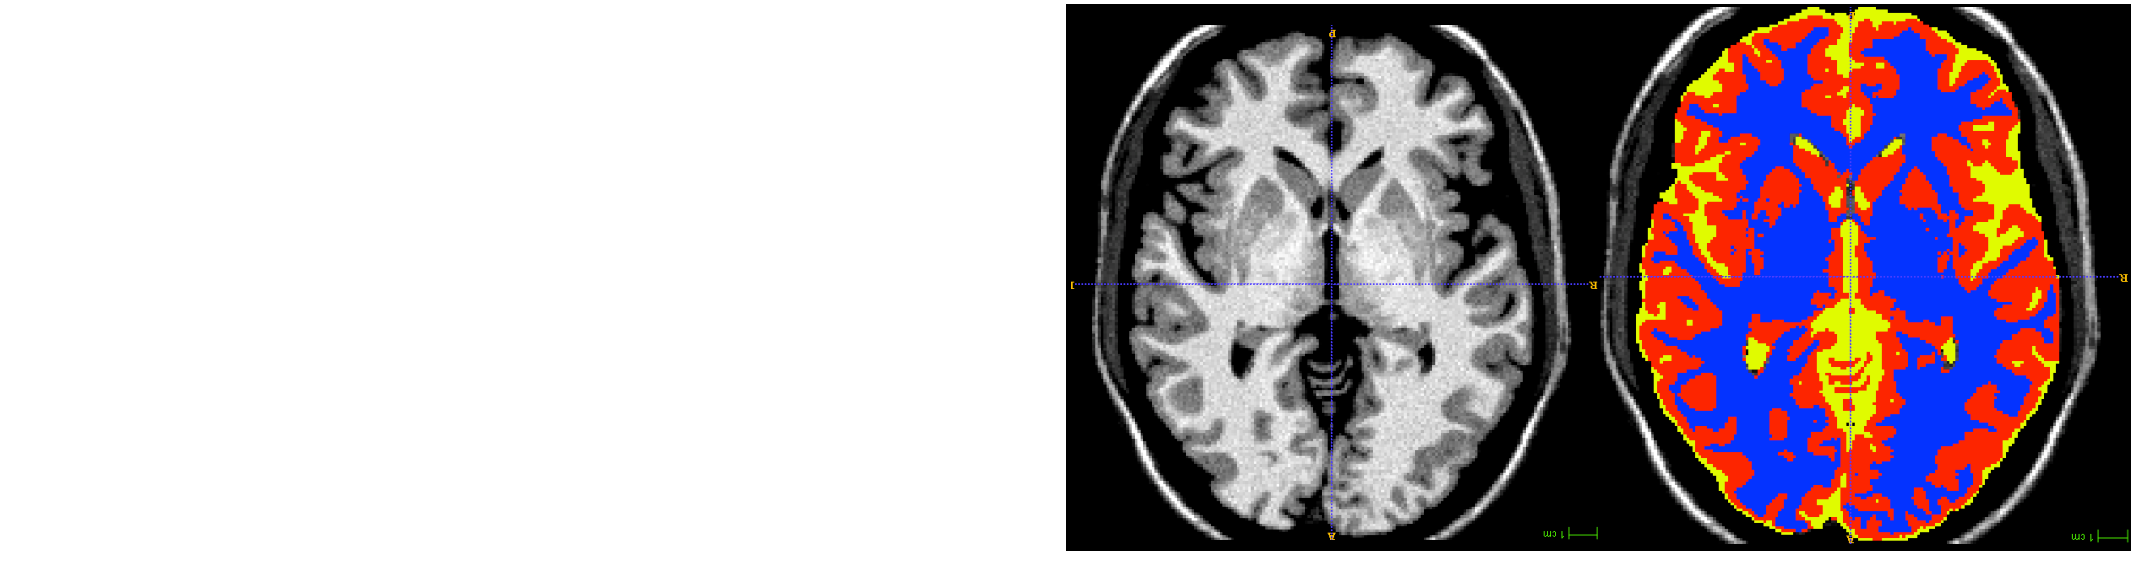
\includegraphics[height=20mm]{atropos.pdf} \\
N4 bias correction \cite{Tustison2010} & Atropos $n$-tissue segmentation \cite{Avants2011a} \\  
\vspace{-1mm}\\
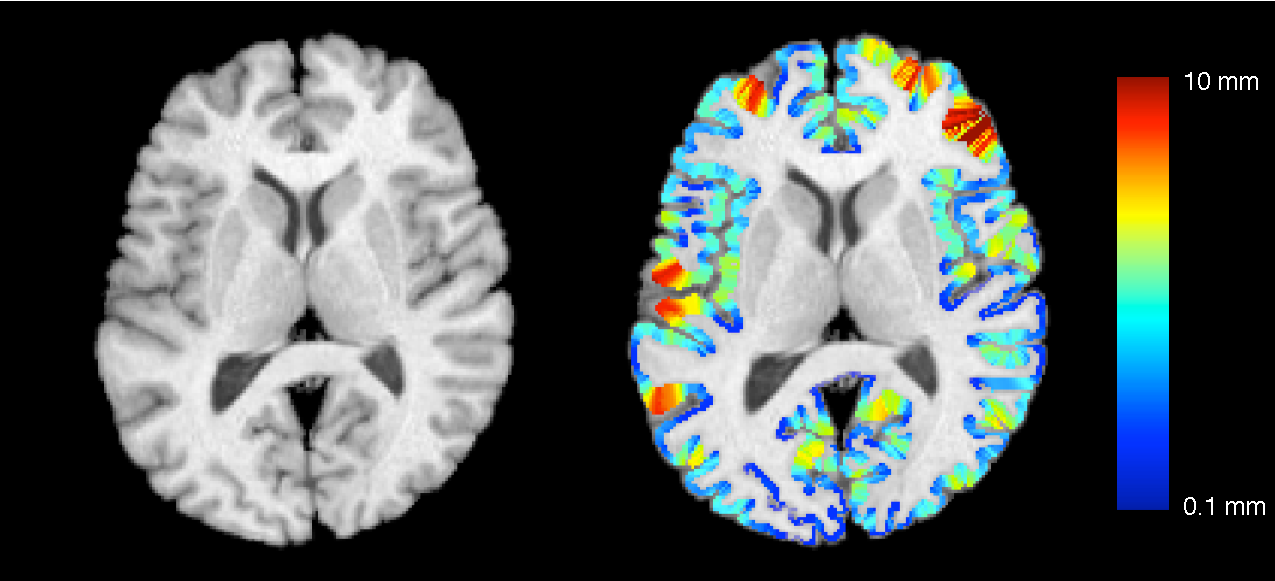
\includegraphics[height=20mm]{r16.pdf} & 
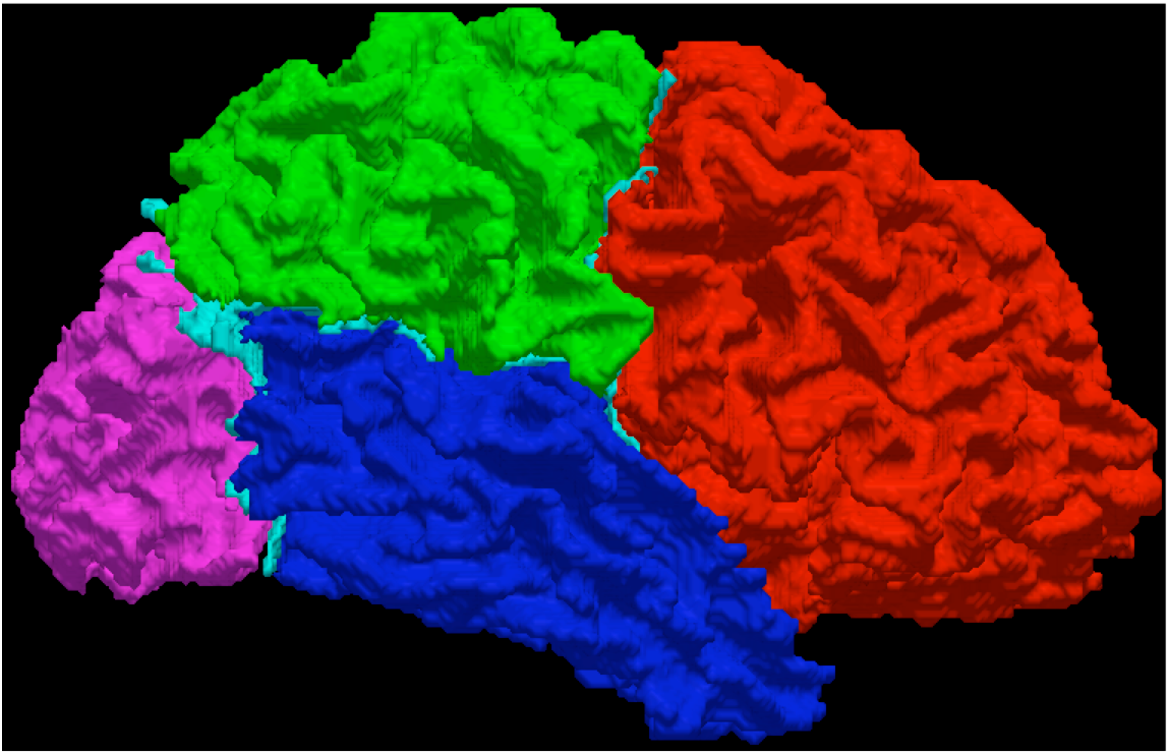
\includegraphics[height=20mm]{glamglue.pdf} \\
DiReCT cortical thickness \cite{Das2009} & topological well-composedness \cite{Tustison2011} \\
\vspace{-1mm}\\
\end{tabular}
\end{center}

\vspace{-6mm}

\begin{center}
{\bf Multivariate analysis using SCCA}\\
\end{center}
\vspace{-1mm}
Sparse canonical correlation analysis (SCCA) adapts classical CCA to
situations where the number of predictors is much greater than the number
of subjects for inference of correlative relationships between different
``views'' of some underlying phenomenon. For gray matter density ($\mathbf{G}$) and
DTI-derived  ($\mathbf{F}$) views, SCCA solves the following
criterion \cite{Avants2010b}:
\vspace{-7mm}
\begin{center}
\begin{align*}
\underset{\omega_{\mathbf{G}}, \omega_{\mathbf{F}}}{\operatorname{argmax}} \left\{\omega_{\mathbf{G}} \mathbf{G}^\mathrm{T}\mathbf{F}\omega_{\mathbf{F}} - \lambda_{\mathbf{G}}\sum_{v_{\mathbf{G}}} |\omega_{\mathbf{G}}|_1 - \lambda_{\mathbf{F}}\sum_{v_{\mathbf{F}}} |\omega_{\mathbf{F}}|_1\right\}: \|\omega_{\mathbf{G}}\|, \|\omega_{\mathbf{F}}\| \leq 1.
\end{align*}
\end{center}

%\smaller
%\begin{center}
%  http://wwww.picsl.upenn.edu/ANTs
%\end{center}  

%\vspace{0.3em}
  }


%%%%%%%%%%%%%%%%%%%%%%%%%%%%%%%%%%%%%%%%%%%%%%%%%%%%%%%%%%%%%%%%%%%%%%%%%%%%%%
  \headerbox{Materials and methods:  ANTs subject and template processing}{name=workflow,column=1,span=2}{
%%%%%%%%%%%%%%%%%%%%%%%%%%%%%%%%%%%%%%%%%%%%%%%%%%%%%%%%%%%%%%%%%%%%%%%%%%%%%%
  \vspace{0.3em}

\begin{center}
\begin{tabular}{p{11cm}p{11cm}}
{\makebox[11cm][c]{\bf Individual subject processing}\vspace{-3mm} } & 
{\makebox[11cm][c]{\bf Template generation}} \\
{\makebox[11cm][c]{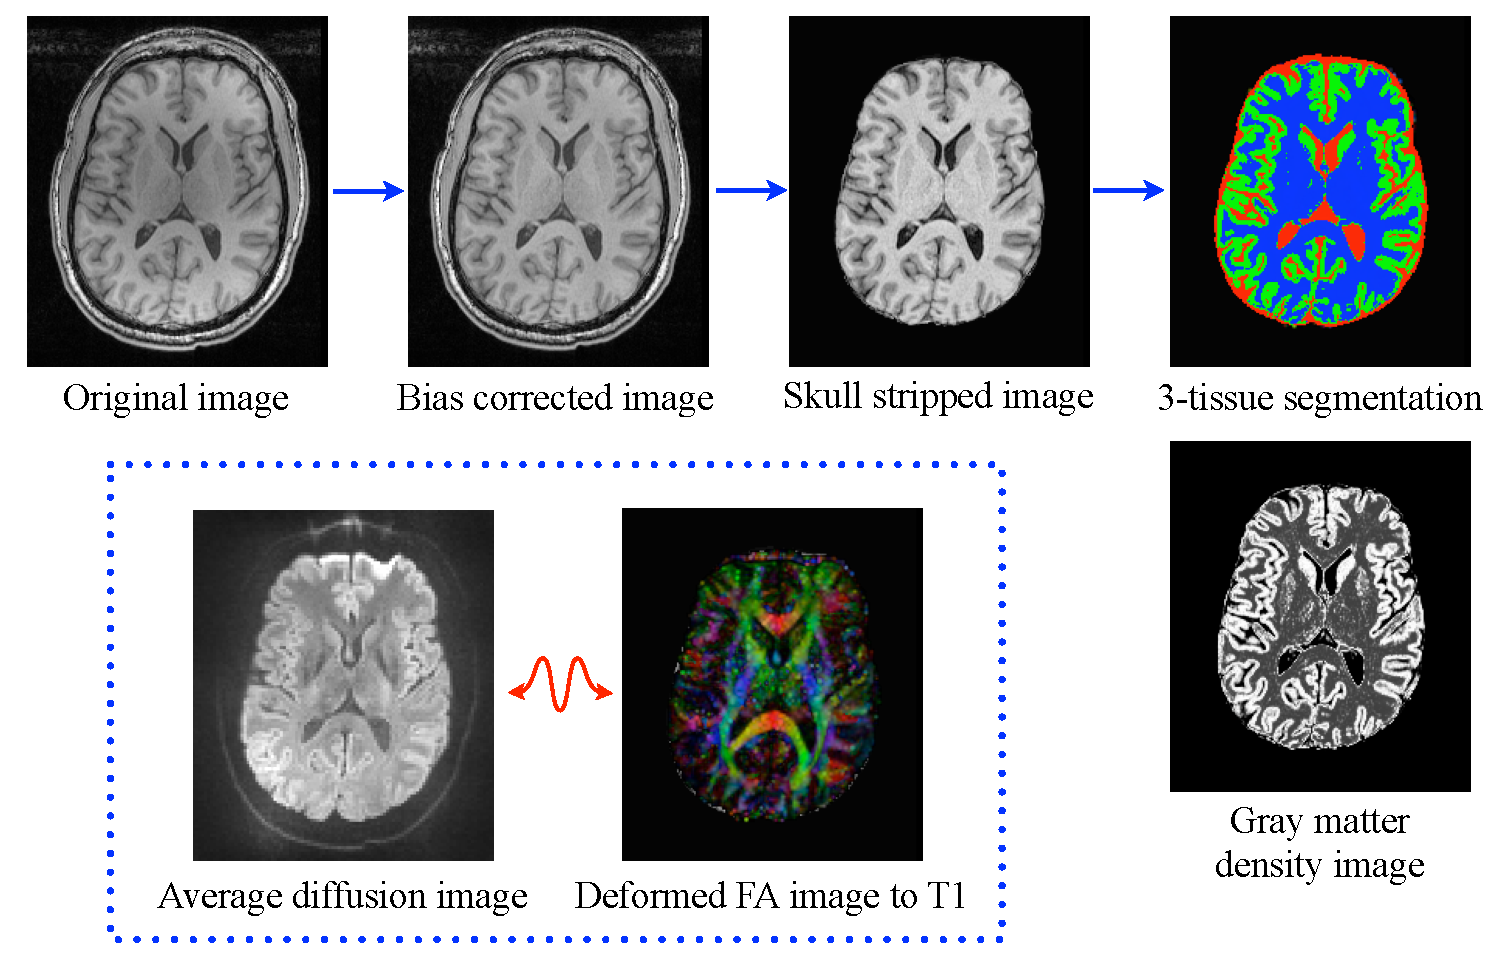
\includegraphics[height=60mm]{individualProcessing.pdf}}}\vspace{3mm} &
{\makebox[11cm][c]{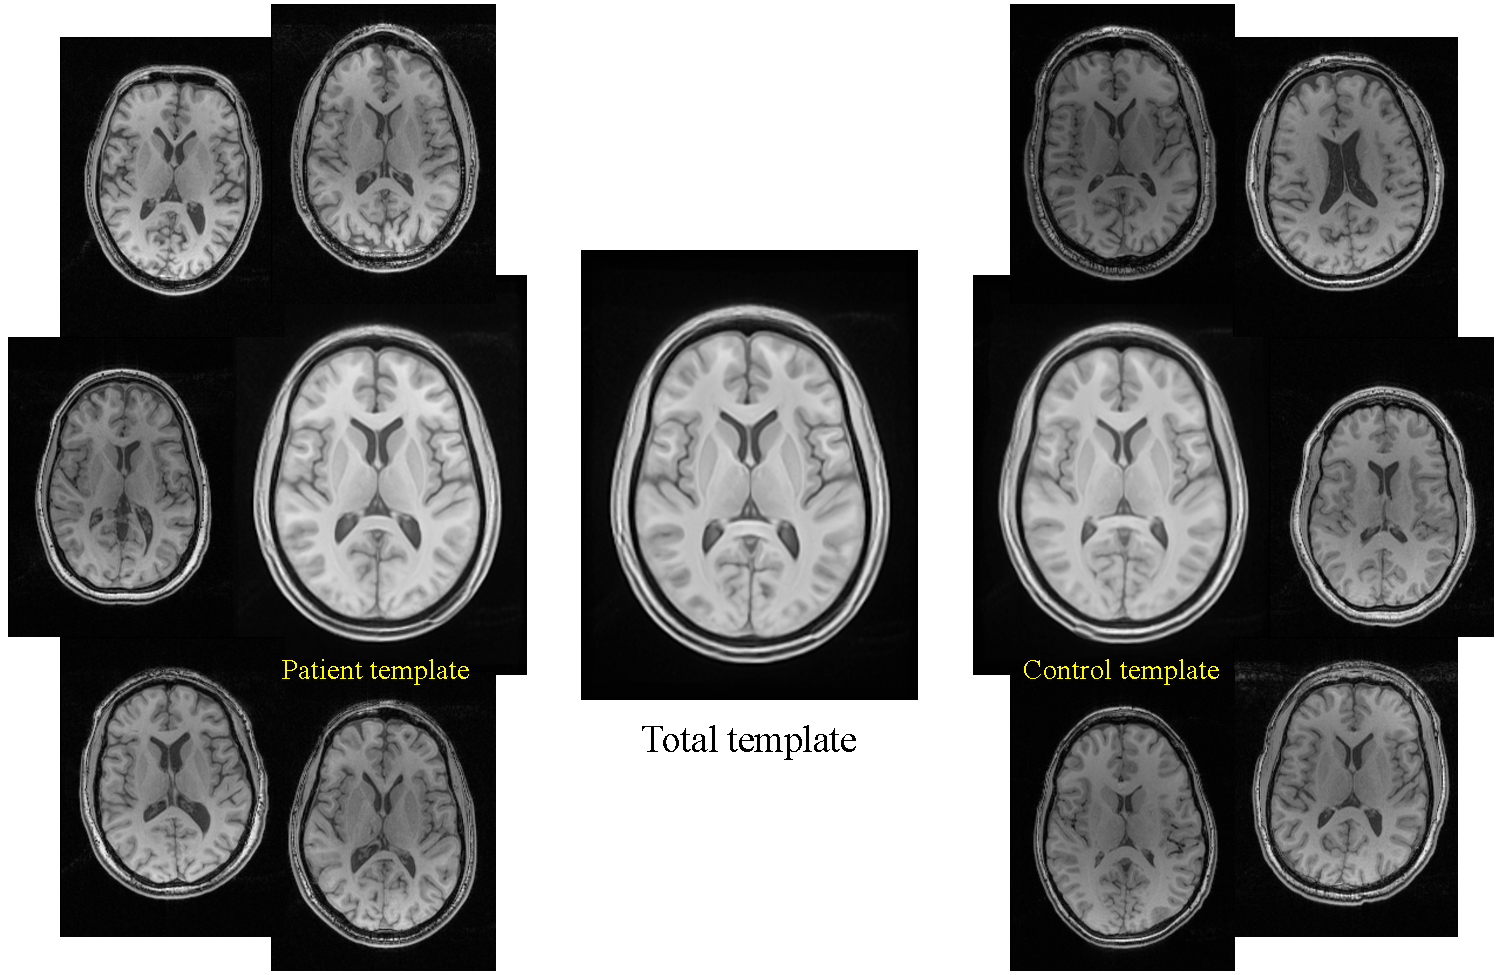
\includegraphics[height=60mm]{templateBuilding.pdf}}} \\
\small Processing of each anatomical (T1-weighted) image consists of the
following steps: 
\begin{itemize}
  \item bias correction,
  \item skull stripping using Atropos coupled with anatomical priors, and
  \item prior-based cerebrospinal fluid, white and gray matter segmentation.  The
  latter yields the gray matter density (GMD) image for each subject.
\end{itemize}
DTI-derived fractional anisotropy (FA) images are mapped to each anatomical image using the transform
obtained from registration of the average diffusion image to the 
corresponding T1. 
& 
\small Statistical analysis requires normalization to a standard space provided
by the total template.  All 17 controls and all 16 TBI patients were used
to generate their respective unbiased templates.  These two templates were then
used to generate the final/standard template.  Thus the mapping from the individual 
GMD image to the total template is given by
\begin{align*}
  \mathrm{GMD}_{subject}\,\,\mathbf{Id}\,\, \mathrm{T1}_{subject}\leadsto \mathrm{template}_{population}\leadsto \mathrm{template}_{total}.
\end{align*}
Similarly, the mapping for each subject's FA image to the total template is given
by the 
transform composition
\begin{align*}
  \mathrm{FA}_{subject}\rightarrow\mathrm{T1}_{subject}\leadsto \mathrm{template}_{population}\leadsto \mathrm{template}_{total}.
\end{align*}
\\
\end{tabular}
\end{center}

\vspace{-10mm}
  }

%%%%%%%%%%%%%%%%%%%%%%%%%%%%%%%%%%%%%%%%%%%%%%%%%%%%%%%%%%%%%%%%%%%%%%%%%%%%%%
  \headerbox{Multivariate analysis results}{name=results,column=1,span=2,below=workflow}{
%%%%%%%%%%%%%%%%%%%%%%%%%%%%%%%%%%%%%%%%%%%%%%%%%%%%%%%%%%%%%%%%%%%%%%%%%%%%%%
  \vspace{0.3em}

\begin{center}
\begin{tabular}{p{6cm}cc} \vspace{-70mm}
{\makebox[6cm][c]{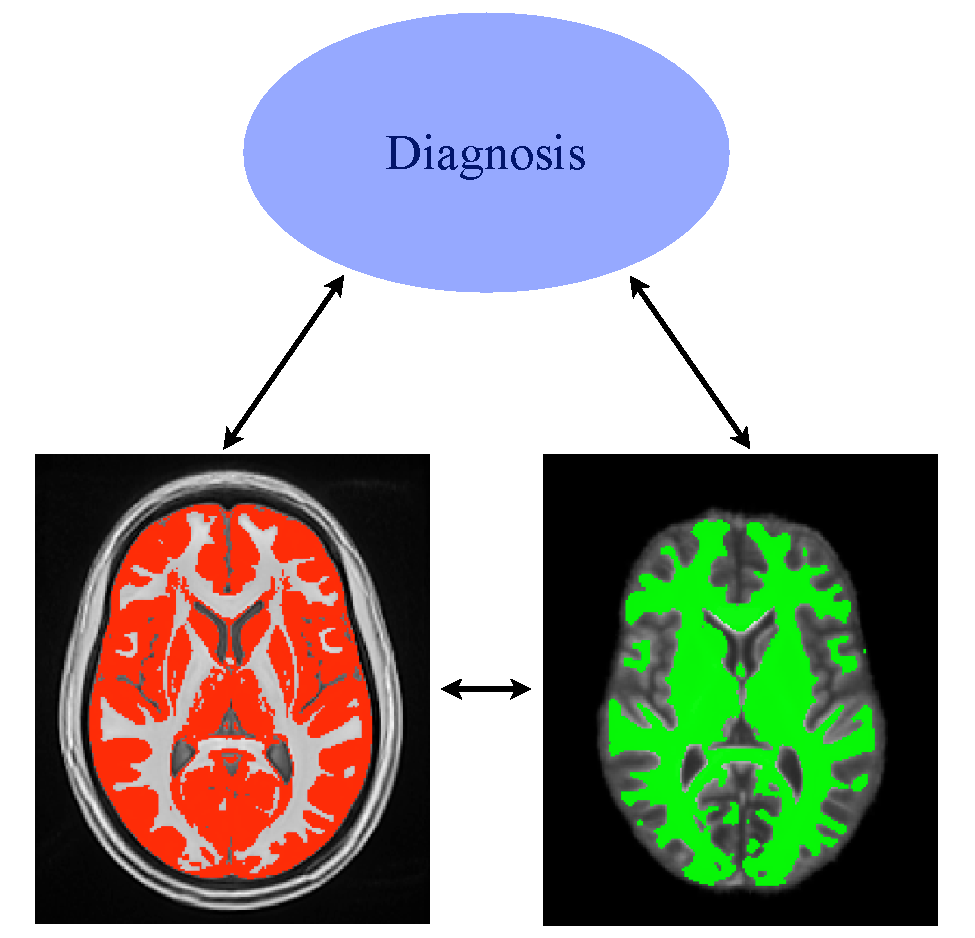
\includegraphics[height=50mm]{scca.pdf} }} \
\small The significant correlations derived from the GMD/FA views
vs. diagnostic view provide significant regions for finding
correlations between GMD and FA. & {           } &
{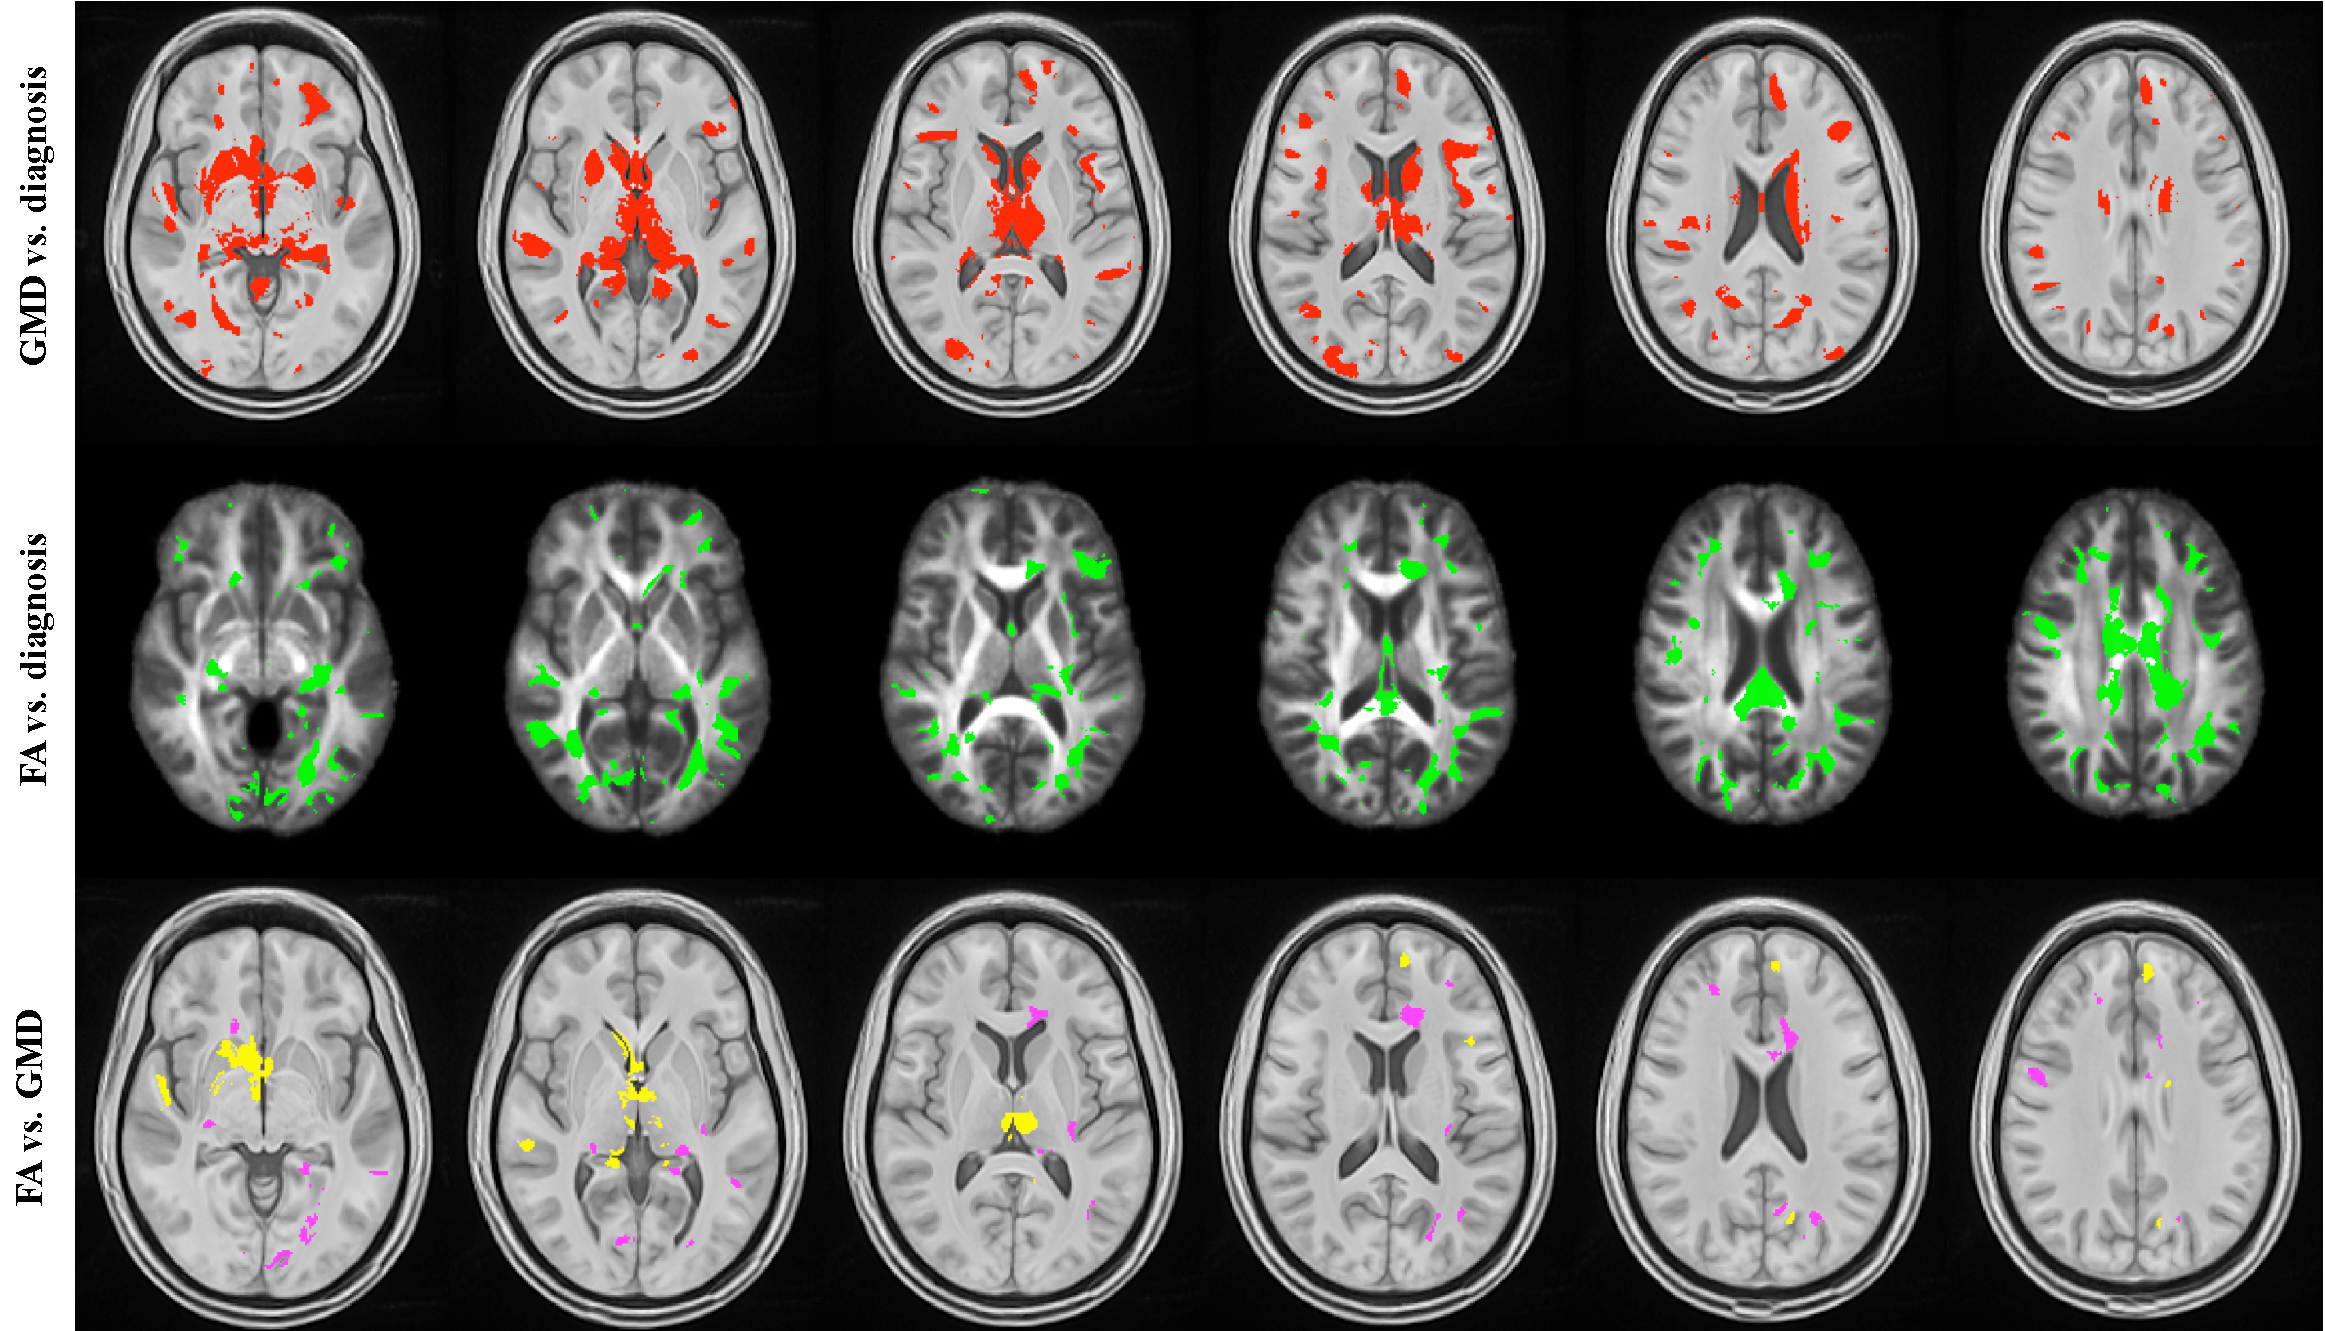
\includegraphics[height=80mm]{resultsPartial.pdf}}
\end{tabular}
\end{center}

  }

%%%%%%%%%%%%%%%%%%%%%%%%%%%%%%%%%%%%%%%%%%%%%%%%%%%%%%%%%%%%%%%%%%%%%%%%%%%%%
  \headerbox{Conclusions}{name=conclusions,column=1,below=results}{
%%%%%%%%%%%%%%%%%%%%%%%%%%%%%%%%%%%%%%%%%%%%%%%%%%%%%%%%%%%%%%%%%%%%%%%%%%%%%

 SCCA demonstrates significant differences between the control and patient groups in both the FA ($p < 0.002$) and gray matter ($p < 0.04$)	that	are	widespread 	but	largely	focus	on	 thalamocortical networks related to the limbic system. Specific regional differences included the medial thalamic nuclei, hypothalamus, amygdala, hippocampus, anterior cingulate cortex, orbitofrontal cortex and fornix. Using these SCCA-identified regions, we demonstrate a strong correlation ($p < 0.01$) of the degree of injury in WM and GM within the patient group.
 
\vspace{0.3em}
  }

%%%%%%%%%%%%%%%%%%%%%%%%%%%%%%%%%%%%%%%%%%%%%%%%%%%%%%%%%%%%%%%%%%%%%%%%%%%%%
  \headerbox{References}{name=references,column=2,below=results,above=bottom}{
%%%%%%%%%%%%%%%%%%%%%%%%%%%%%%%%%%%%%%%%%%%%%%%%%%%%%%%%%%%%%%%%%%%%%%%%%%%%%

\vspace{2mm}
    \tiny % \scriptsize
      \vspace{-0.4em}
      \renewcommand{\refname}{\vspace{-0.8em}}
      \bibliographystyle{abbrv}
      \bibliography{references}

  \begin{center}
  {\small \bf Open source software} \\
{\vspace{3mm}}
  \begin{tabular}{cc}
  
\includegraphics[height=12mm]{ants_logo.png} &
  
\includegraphics[height=11mm]{itkLogo.jpg} \\
%  {Advanced Normalization Tools} & {Insight Toolkit} \\
  {\tiny http://www.picsl.upenn.edu/ANTs} &
%  {\tiny http://www.cs.ucl.ac.uk/research/medic/camino} &
  {\tiny http://www.itk.org/} \\
  \end{tabular}
  \end{center}


%    \bibliographystyle{ieee}
%    \renewcommand{\section}[2]{\vskip 0.05em}
%      \begin{thebibliography}{1}\itemsep=-0.01em
%      \setlength{\baselineskip}{0.4em}
%      \bibitem{amberg07:nonrigid}
%        B.~Amberg, S.~Romdhani, T. Vetter.
%        \newblock {O}ptimal {S}tep {N}onrigid {ICP} {A}lgorithms for {S}urface {R}egistration
%        \newblock In {\em Computer Vision and Pattern Recognition 2007}
%      \bibitem{amberg08:recognition}
%        B.~Amberg, R.~Knothe, T. Vetter.
%        \newblock Expression Invariant Face Recognition with a 3D Morphable Model
%        \newblock In {\em Automated Face and Gesture Recognition 2008}
%      \end{thebibliography}
  }


%%%%%%%%%%%%%%%%%%%%%%%%%%%%%%%%%%%%%%%%%%%%%%%%%%%%%%%%%%%%%%%%%%%%%%%%%%%%%
  \headerbox{Acknowledgments}{name=acknowledgments,column=1,below=conclusions,above=bottom}{
%%%%%%%%%%%%%%%%%%%%%%%%%%%%%%%%%%%%%%%%%%%%%%%%%%%%%%%%%%%%%%%%%%%%%%%%%%%%%
  \vspace{1mm}
  \smaller
   Partial funding support was provided by US ARMY Medical Research
   and Materiel Command grant W81XWH-09-2-0055.
   This project is also funded, in part, under a grant with the Pennsylvania 
  Department of Health. The Pennsylvania Department of Health specifically disclaims responsibility 
  for any analyses, interpretations, or conclusions.
  }

%%%%%%%%%%%%%%%%%%%%%%%%%%%%%%%%%%%%%%%%%%%%%%%%%%%%%%%%%%%%%%%%%%%%%%%%%%%%%%%
%  \headerbox{Expression Neutralization}{name=results neutralization,column=1,row=0}{
%%%%%%%%%%%%%%%%%%%%%%%%%%%%%%%%%%%%%%%%%%%%%%%%%%%%%%%%%%%%%%%%%%%%%%%%%%%%%%%
%  \begin{tikzpicture}[x=0.3333\linewidth,y=-0.42\linewidth]
%    \path [use as bounding box] (-0.5,-0.5) rectangle(2.5,1.7);
%    \path
%    (0,0) node{\includegraphics[width=0.42\linewidth]{D1077}}
%    (1,0) node{\includegraphics[width=0.47\linewidth]{D1077_fit_expression}}
%    (2,0) node{\includegraphics[width=0.47\linewidth]{D1077_fit}}
%
%    (0,1) node{\includegraphics[width=0.42\linewidth]{D1360}}
%    (1,1) node{\includegraphics[width=0.47\linewidth]{D1360_fit_expression}}
%    (2,1) node{\includegraphics[width=0.47\linewidth]{D1360_fit}}
%
%    (0,1.6) node {\smaller a) Target}
%    (1,1.6) node {\smaller b) Fit}
%    (2,1.6) node {\smaller c) Normalized};
%  \end{tikzpicture}
%  \vspace{0.5em}
%
%  Expression normalisation for two scans of the same individual.  
%  The robust fitting gives a good estimate (b) of the true face surface given
%  the noisy measurement (a). It fills in holes and removes artifacts using
%  prior knowledge from the face model. The pose and expression normalized faces
%  (c) are used for face recognition.
%  \vspace{0.5em}
%  }
%%%%%%%%%%%%%%%%%%%%%%%%%%%%%%%%%%%%%%%%%%%%%%%%%%%%%%%%%%%%%%%%%%%%%%%%%%%%%%%
%  \headerbox{Funding}{name=funding,column=1,span=2,above=bottom}{
%%%%%%%%%%%%%%%%%%%%%%%%%%%%%%%%%%%%%%%%%%%%%%%%%%%%%%%%%%%%%%%%%%%%%%%%%%%%%%%
%  \smaller 
%  \hspace{1em}This work was supported in part by Microsoft Research through the European PhD Scholarship Programme.
%  }
%%%%%%%%%%%%%%%%%%%%%%%%%%%%%%%%%%%%%%%%%%%%%%%%%%%%%%%%%%%%%%%%%%%%%%%%%%%%%%%
%  \headerbox{Robustness}{name=robustness,column=2,row=0,above=results,span=1}{
%%%%%%%%%%%%%%%%%%%%%%%%%%%%%%%%%%%%%%%%%%%%%%%%%%%%%%%%%%%%%%%%%%%%%%%%%%%%%%%
%  \begin{tikzpicture}[x=0.3333\linewidth,y=-0.42\linewidth]
%    \path [use as bounding box] (-0.5,-0.5) rectangle(2.5,1.7);
%    \path
%    (0,0) node{\includegraphics[width=0.42\linewidth]{D1160}}
%    (1,0) node{\includegraphics[width=0.42\linewidth]{D1425}}
%    (2,0) node{\includegraphics[width=0.42\linewidth]{D1205}}
%
%    (0,1) node{\includegraphics[width=0.28\linewidth]{D1160_fit_expression}}
%    (1,1) node{\includegraphics[width=0.28\linewidth]{D1425_fit_expression}}
%    (2,1) node{\includegraphics[width=0.28\linewidth]{D1205_fit_expression}}
%
%    (1,0.5) node {\smaller a) Target}
%    (1,1.6) node {\smaller b) Robust Reconstruction};
%  \end{tikzpicture}
%  \vspace{0.5em}
%
%  The reconstruction (b) is robust against scans (a) with artifacts, noise, and
%  holes.
%  
%  This is achieved by a robust iteratively reweighted ICP algorithm and outlier
%  rejection based on angle comparisions between corresponding points.
%  }


\end{poster}

\end{document}
